%%%%%%%%%%%%%%%%%%%%%%%%%%%%%%%%%%%%%%%%%%%%%%%%%%%%%%%%%%%
% Zusammenfassung des Logbuchs - Florian Adamczyk
% KI 1 Projekt, WS 2025/26 - Gruppe 308
%%%%%%%%%%%%%%%%%%%%%%%%%%%%%%%%%%%%%%%%%%%%%%%%%%%%%%%%%%%

\documentclass[9pt,a4paper,twocolumn,twoside]{tau-class/tau}
\usepackage[ngerman]{babel}
\usepackage{booktabs}
\usepackage{siunitx}
\usepackage{pdfpages}
\usepackage{hyperref}
\begin{document}
	
%%%%%%%%%%%%%%%%%%%%%%%%%%%%%%%%%%%%%%%%%%%%%%%%%%%%%%%%%%%%%%%%%%%%%%%%%%%%%%%%%%%%%%%%%

\begin{titlepage}
    \centering
    \vspace*{0.5 cm}
    % \begin{large} Justus-Liebig-Universität\\ Gießen \end{large}
    
\includegraphics[width = 0.6 \textwidth]{figures/JLU_Giessen-Logo}	%University Logo
    \\[2.0 cm]
    % \begin{center}    \textsc{\Large Justus - Liebig - Universität}\\{Giessen}\\[0.8cm]	\end{center}% University Name
    
    \textsc{\Large Gruppennummer: 308}  \\[0.3 cm]				% Course Code
    \rule{\linewidth}{0.2 mm} \\[0.2 cm]
    { \huge \bfseries Neuronales Netz f\"ur den kalifornischen Hauspreis-Datensatz}\\
    \rule{\linewidth}{0.2 mm}\\[2.0 cm]
    
    
    \begin{minipage}{0.5\textwidth}
        \begin{flushleft}
            \emph{Übrige Gruppenmitglieder:}\\
            \large{Florian Adamczyk}\\
            \large{Björn Becker}\\
            \large{Felix Hollfoth (Sprecherin)}\\
            \large{Kolja Scriba}\\
            %  Affiliation\\
        \end{flushleft}
    \end{minipage}~
    \begin{minipage}{0.5\textwidth}
        \begin{flushright}
            
            \emph{Protokoll von:} \\
            
            \large{Felix Neumann (Sprecherin)}\\ 
            \small{\href{mailto:felix.neumann@stud.uni-giessen.de}{felix.neumann@stud.uni-giessen.de}\\
                Matrikel Nr.: 16639\: }\\[0.5cm]
            
        \end{flushright}
    \end{minipage}\\[2.0 cm]

        
    \begin{minipage}{0.8\textwidth}
       \begin{center}
        \large
        Modul: Künstliche Intelligenz I\\
        Dozent: Prof. Dr. Christian Heiliger\\
        Semester: Wintersemester 2025/26
        \end{center} 
    \end{minipage}

\vfill

\end{titlepage}







%----------------------------------------------------------
% Title & Author
%----------------------------------------------------------

\doctype{Zusammenfassung des Logbuchs}
\title{Neuronales Netz f\"ur den kalifornischen Hauspreis-Datensatz}

\author[a]{Felix Neumann}
\affil[a]{Justus Liebig Universität, Matrikelnr.\ 116639}

%----------------------------------------------------------
% Document Info
%----------------------------------------------------------

\dates{Gruppe 308 -- KI~I Projekt WS~2025/26}
\footinfo{KI~I Portfolio}
\theday{\today}
\organization{JLU Gießen}
\leadauthor{F.\ Neumann}

%----------------------------------------------------------
% Abstract
%----------------------------------------------------------

\begin{abstract}
Diese Zusammenfassung dokumentiert den individuellen Projektfortschritt basierend auf dem geführten
 Logbuch im Rahmen des KI~I-Projekts zur Vorhersage kalifornischer Hauspreise mittels neuronaler Netze. Das vollständige Logbuch befindet sich im Anhang des Portfolios.
Dabei wurden mehr als akzeptable Ergebnisse erzielt. Mein Anteil, Vorgehen, die Gedankengänge und Problematiken sind hier unvollständig (im Logbuch vollständig) dokumentiert.
Das Bestergebnis meines Neuronalen Netzes auf die Testdaten, übertraf dabei mit einem $R^2$-Score von 0.7958 das der linearen Regression von 0.6326 deutlich.
%Diese Zusammenfassung dokumentiert meinen individuellen Arbeitsprozess im Rahmen des KI~I-Projekts zur Vorhersage kalifornischer Hauspreise mittels neuronaler Netze. Der Schwerpunkt liegt auf der Projektinfrastruktur, der explorativen Datenanalyse sowie der Entwicklung und Evaluation eines TensorFlow/Keras-basierten Regressionsmodells. Das beste neuronale Netz erreicht einen $R^2$-Wert von 0{,}78 auf dem Testset und \"ubertrifft damit die lineare Regression ($R^2 = 0{,}63$) deutlich.
\end{abstract}

\keywords{Neuronales Netz, California Housing, TensorFlow, Regression, Machine Learning}

%----------------------------------------------------------

%\begin{document}

\maketitle
\thispagestyle{firststyle}


%----------------------------------------------------------
%----------------------------------------------------------
%----------------------------------------------------------
\section{Fragestellungen}

\taustart{D}Diese Zusammenfassung dokumentiert den individuellen Projektfortschritt basierend auf dem geführten Logbuch.
Die zentrale Fragestellung der Arbeit lag in der Optimierung neuronaler Netze für den California-Housing-Datensatz und einem anschließenden Vergleich dieser zu der linearen Regression.
Als Zielvariable diente dabei der \textit{MedHouseVal}.
Basierend auf dem Fortschritt der Teammitglieder, in den Bereichen der besten Hyperparameterwahl, sowie der generellen Architektur und
inbesondere der Erkenntnis, dass eine isolierte Hyperparamterwahl nicht zielführend war entstanden verschiedene Ansätze für das Vorgehen.
Neben einer Simultanoptimierung der Hyperparameter die effizienter und Ressourcensparender läuft,
als die bereits erprobten Grid- und Randomsearchvarianten, sollte auch an den Features selbst Veränderungen ausprobiert werden. 
Dabei wurden folgende spezifische Teilfragen untersucht:
\begin{itemize}
    \item Wie lässt sich die Hyperparameter-Suche durch bayesianische Optimierung im Vergleich zu Grid- oder Random-Search effizienter gestalten?
    \item Kann das Netz durch Feature engineering weiter verbessert werden? Welchen Einfluss haben neu generierte Features (wie \texttt{Bedrooms\_per\_Room} oder geografische Distanzen zu Los Angeles und San Francisco) auf die Modellperformance?
    \item Ab welcher \textit{Gini Importance} können Features vernachlässigt werden, ohne dass das neuronale Netz an Vorhersagekraft verliert?
\end{itemize}

%----------------------------------------------------------
\section{Ansätze und Methoden}
\subsection{bayesianische Optimierung}
Zur grundlegenden Orientierung beim Aufbau und der Theorie der neuronalen Netze diente einschlägige Fachliteratur \cite{russell2020ai}.
Die anderen Gruppenmitglieder (inbesondere Felix H.) verusuchten zunächst durch isolierte Hyperparameterwahl sinnvolle Zusammensetzungen
für die Architektur zu finden. Später erfolgte eine zielgerichtete suche mit Grid- und Randomsearch.
Da diese sehr zeitaufwändig nach leistungsfähigen Hyperparameterzusammensetzungen suchten, recherchierte ich weitere Möglichkeiten zur Beschleunigung des Vorganges.
Als Resultat wurde die bayesianische Optimierung mittels \texttt{KerasTuner} \cite{kerastuner2019} implementiert.
Dieser Ansatz wählt Hyperparameter basierend auf vergangenen Trainingsläufen aus, was die Rechenzeit drastisch reduziert hat.
Zunächst wurden einfache, flache sequentielle Modelle \cite{keras_sequential} trainiert, um das Risiko von Vanishing Gradients und Overfitting zu minimieren.
Im weiteren Verlauf wurde die Breite der Netzwerke auf bis zu 256 Neuronen erweitert und Regularisierungstechniken wie Dropout sowie die \texttt{LeakyReLU}-Aktivierungsfunktion getestet.
Auch mit verschiedenen Tiefen wurden experimentiert. Zum Schluss erlangte das beste Ergebnis ein Netz mit drei Hidden Layern und einer batch-size von 32,
wie sie erfolgreich durch die Kommolitonen als geeignet ermittelt wurde.
Versuche mit größeren Batchsizes wurden zwar durchgeführt, gingen jedoch bei allen Versuchen zulasten des $R^2-Score$.
Zudem kam ein dynamischer Learning-Rate-Scheduler in Verbindung mit \cite{early_Stopping} und der Adam-Optimizer zum Einsatz. Anhand des Plot "\figref{fig:Loss}" lässt sich sehr gut die Funktion des eingesetzten Earlystoppings während eines 
beispielhaften Modelldurchlaufs erkennen.


\subsection{Feature Engineerings}
Zunächst erfolgte eine allgemeine Featureanalyse. Ganz klar zu erkennen ist die dominanz des Medium Income Features
bei einem Vergleich der Featureimportances. Es drängte sich die Frage auf, ob aus den restlichen Features noch mehr Information zu gewinnen sei.
Durch eine Division der Features \texttt{AveBedrms} und \texttt{AveRooms} errechnete ich das Feature \texttt{Bedrooms\_per\_Room}.
Die Analyse der aktuellen Wohnraumpreise in Kalifornien zeigte eine klare Tendenz hoher Kosten in der 
Nähe von Los Angeles und San Francisco. Die Frage war nun, ob dies auch aus dem Datensatz mit Daten der 90er hervor geht.
 Aus den vorhanden Features für Längen und Breitengrad konnte jeweils ein 
Feature für die relative Nähe zu den beiden Großstädten ermittelt werden. 
Zusätzlich wurden diese auch noch auf einfache Weise verrechnet und ein weiteres geografisches Feature \texttt{Lat\_x\_Lon} konnte hinzugefügt werden.
Eine weitere Feststellung war die rechtsschiefe Verteilung der Population. Da neuronale Netze mit schiefen Verteilungen etwas Schwierigkeiten
haben können, wurde Testweise eine lorathmische Betrachtung \texttt{log\_Population}. 
Zur Evaluation dieser methodischen Anpassungen wurde ein Random-Forest-Regressor trainiert, um die \textit{Feature Importance} \figref{fig:feature_importance} zu analysieren und irrelevante Merkmale zu identifizieren.
Die Korrelation zur Zielvariablen kann durch eine \figref{fig:correlation_heatmap} abgelesen werden. 
Darauf zu erkennen ist die Dominanz der Korrelation des Median Einkommens zur Zielvariable, sowie eine nichttriviale Korrelation der neu eingeführten
Distanz Features \texttt{Dist\_to\_SF} und \texttt{Dist\_to\_LA}.
\begin{figure}[htbp]
    \centering
    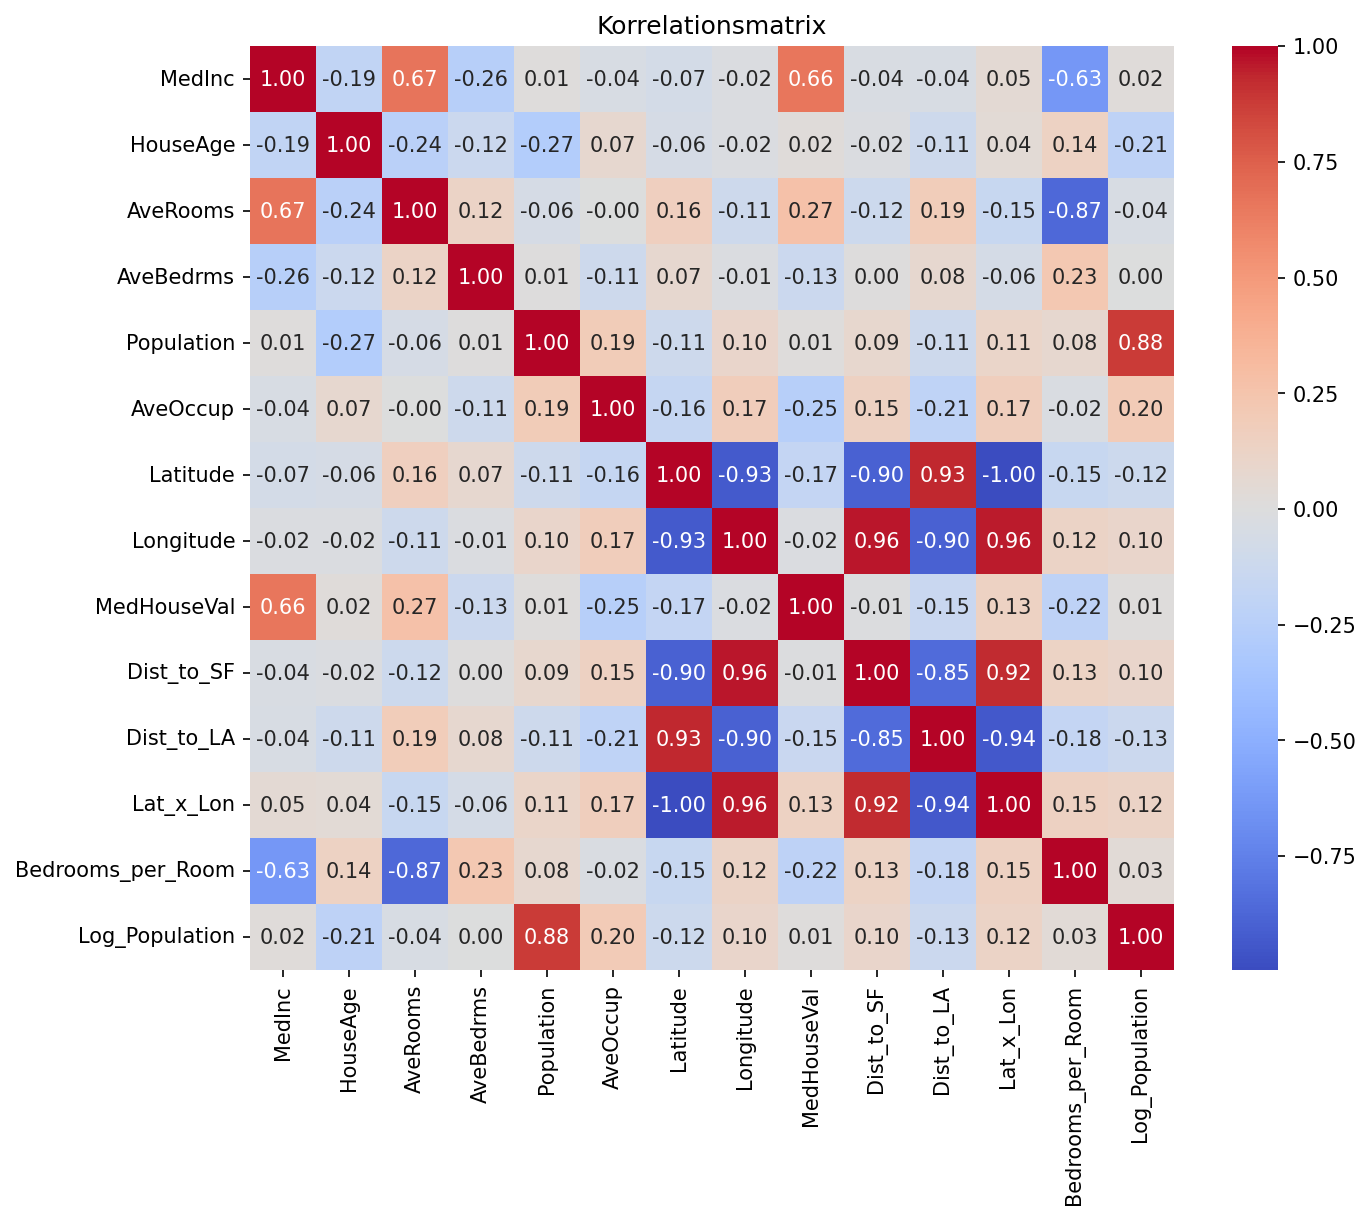
\includegraphics[width=0.95\columnwidth]{figures/eda_correlation_heatmap.png}
    \caption{Korrelationskarte}
    \label{fig:correlation_heatmap}
\end{figure}
%----------------------------------------------------------
\section{Ergebnisse}
Der Plot "\figref{fig:Beispiel Historgramm}" dient als Beispielresiduenverteilung aller erstellter Modelle.
 Diese unterscheiden sich nur unwesentlich und haben alle eine sehr ähnliche Veteilung. 
\begin{figure}[H]
    \centering
    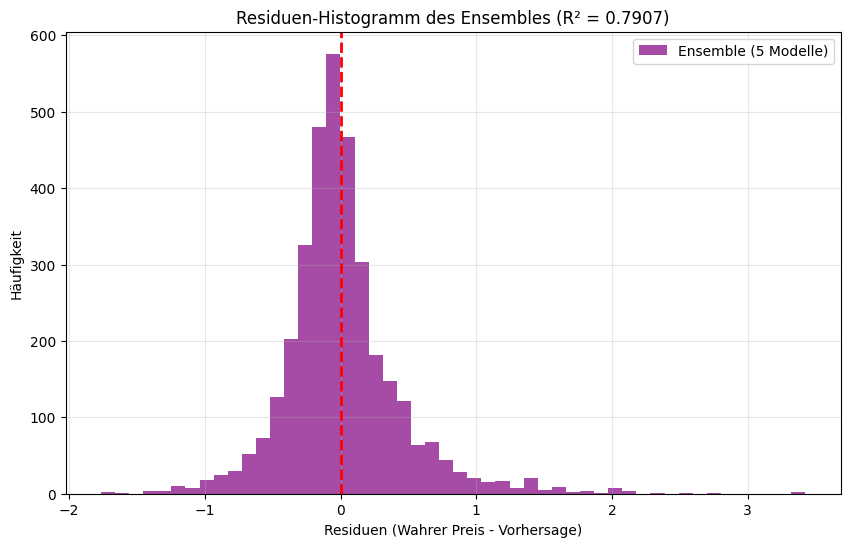
\includegraphics[width=0.95\columnwidth]{figures/Beispiel_Resi_Hist.png}
    \caption{Beispiel eines Residuenhistogramms}
    \label{fig:Beispiel Historgramm}
\end{figure}
Das Residuendiagramm zeigt eine Zentrierung der Werte um die Nulllinie. Das Modell hat demnach keinen systematischen Bias und unterschätzt Werte ähnlich oft, wie es sie überschätzt.   
Obgleich der Großteil des Fehlers in einem engen Bereich liegt, zeigt er keine perfekte Normalverteilung, sondern hat "heavy tails".
Eine solche leicht Rechtsschiefe Verteilung bedeutet, dass die Preise der Häuser im Zweifel leicht unterschätzt werden.  
Es sind auch einige Outlier (Residuen>2) zu erkennen deren Preis massiv unterschätzt wurde. Dies könnte an dem Fehlen von Features liegen, welche diese Preissteigungen erklären könnten.

\begin{figure}[htbp]
    \centering
    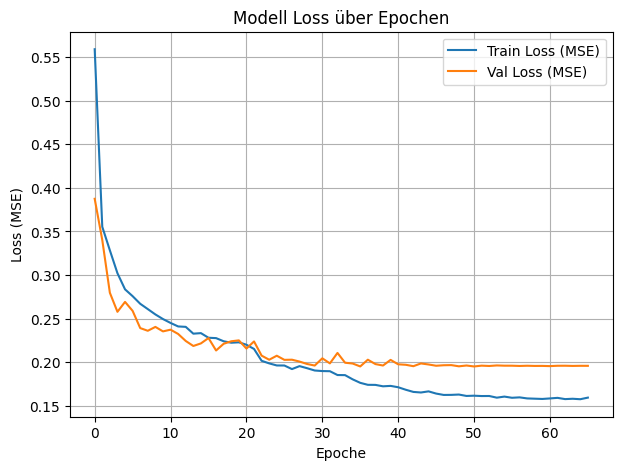
\includegraphics[width=0.95\columnwidth]{figures/Modell_Loss-Plot.png}
    \caption{Loss über die Verschiedenen Epochen}
    \label{fig:Loss}
\end{figure}
Anhand des Plot "\figref{fig:Loss}"  lässt sich sehr gut die Funktion des eingesetzten Earlystoppings während eines 
beispielhaften Modelldurchlaufs erkennen. Das Modell benötigt oft bei weitem nicht alle Epochen für eine Konvergenz. 
Earlystopping bricht den Vorgang bei zu wenig Veränderung verfrüht ab und ermöglicht so eine große Zeitersparnis. 
Darüber hinaus lässt sich ein mit Anzahl der Epochen zunehmend großer Overfitting Gap erkennen.
Der Loss auf den Trainingsdaten verbessert sich vortlaufend während der Loss auf den Testdaten stagniert.

Die bayesianische Optimierung lieferte bei deutlich geringerer Rechenzeit eine vergleichbare Performance wie Random- und Grid-Search.
Sie wurde im folgenen auch für die Ermittlung der Parameter der Netze mit angepassten Features eingesetzt.
Die  Hinzunahme der geografischen Features und \texttt{Bedrooms\_per\_Room} führte zu keiner direkten Verbesserung der Konvergenz oder des $R^2$-Wertes.
Die Feature-Importance-Analyse zeigte zudem, dass populationsbasierte Features am schwächsten abschnitten (vgl.\figref{fig:feature_importance}).
\begin{figure}[htbp]
    \centering
    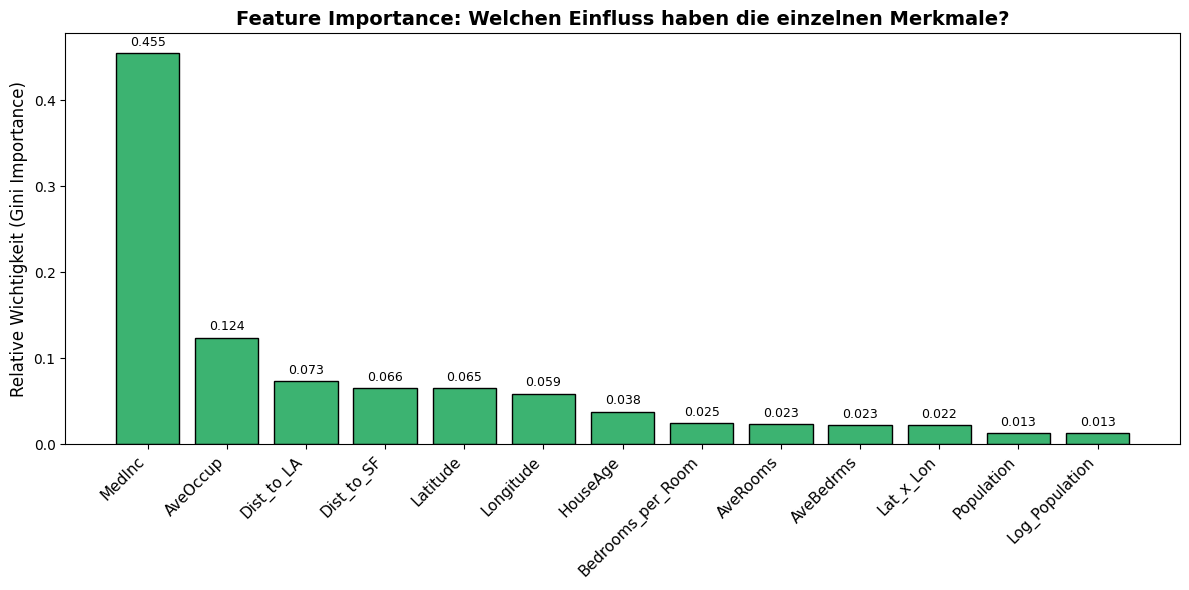
\includegraphics[width=0.95\columnwidth]{figures/Feature importance (with distance features).png}
    \caption{Feature Importance Analyse (inkl. Distanz-Features). Die Grafik verdeutlicht den verhältnismäßig geringen Einfluss der Populations-Features im Vergleich zum Medianeinkommen.}
    \label{fig:feature_importance}
\end{figure}
Ebenfalls zu erkennen ist eine hohe Featureimportance der beiden eingeführten Distanz Features. Dennoch verbesserte sich der $R^2$-Wert durch diese Einführung nicht unmittelbar.
Ein anschließender Versuch, das Netz ohne die schwächsten Features zu trainieren, resultierte in einem verschlechterten $R^2$-Wert von 0{.}783.
Dies führte zu der Erkenntnis, dass neuronale Netze auch aus Merkmalen mit geringer Importance wertvolle Signale und Informationen ziehen, die dem Rauschen dieser Features überwiegen, weshalb keine Features beschnitten wurden.
Der Vergleich zeigte auch, dass der Random Forest minimal bessere Ergebnisse ($\Delta_{Baseline} R^2 = 0.0044$) lieferte als das neuronale Netz.
Mein bestes neuronales Netz mit Ensemble-Methode erreichte einen $R^2$-Wert von 0{.}7958 auf den Testdaten (vgl.\figref{fig:best_Network}).
Das Ziel eines $R^2$-Wertes von über 0{.}8, das durch den Vergleich mit einem Random Forest mit gradient boosting erreicht wurde, konnte damit knapp nicht erreicht werden.
\begin{figure}[htbp]
    \centering
    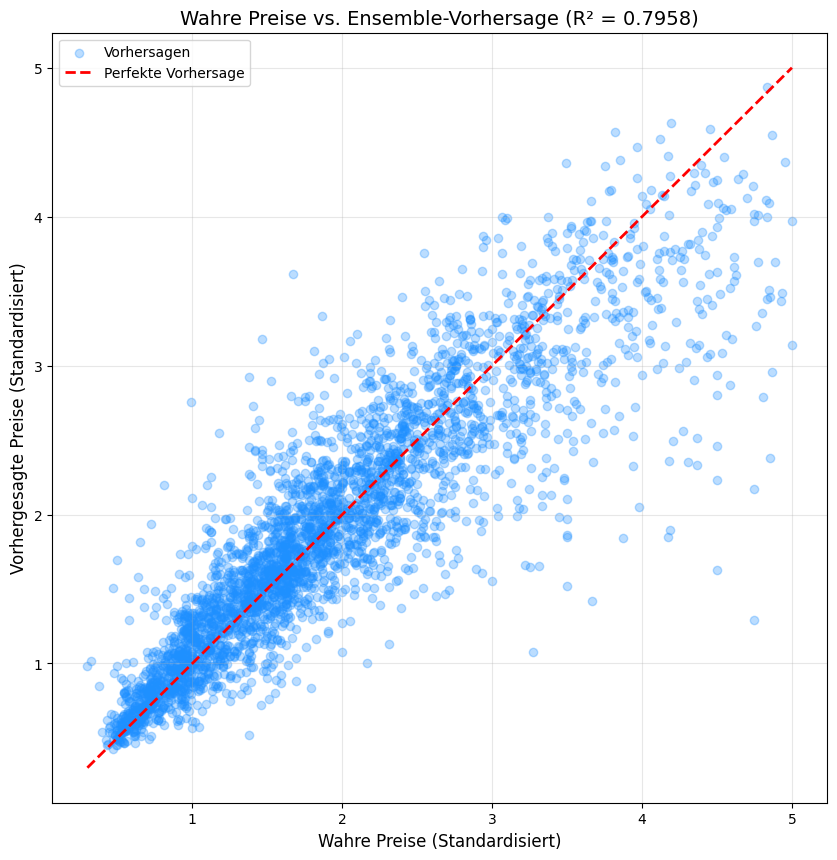
\includegraphics[width=0.75\columnwidth]{figures/stärkstes Modell.png}
    \caption{Das stärkste Neuronale Netz (siehe Vergleich mit linearer Regression)}
    \label{fig:best_Network}
\end{figure}





\subsection{Vergleich mit linearer Regression}
        \begin{table}[H]
        	\caption{Vergleich linearer Regression mit Neuronalem Netz }
        	\label{tab:table}
        	\begin{tabular}{
        		>{\raggedright\arraybackslash}p{0.2\columnwidth}
        		>{\raggedright\arraybackslash}p{0.28\columnwidth}
        		>{\raggedright\arraybackslash}p{0.4\columnwidth}
        	}
        	\toprule
        	\textbf{Metrik} & \textbf{Lineare Regression} & \textbf{Neuronales Netz} \\
        	\midrule
        	$R^2-Score$        & 0.6326  &  0.7958 ($\Delta_{Baseline} R^2 = 0.1632$)       \\
            MAE                & 0.4331  &  0.2895       \\
            RMSE               & 0.5779  &  0.4308        \\
        	\bottomrule
        	\end{tabular}
        	%\tabletext{Note: The table contains data of some famous celestial objects.}
        \end{table}
Das beste in meinem Notebook (und in dem Projekt) erarbeitete Modell zeigt eine deutliche Steigerung gegenüber der Baseline.
Dabei ist zu beachten, dass ein sehr simples Netz die lineare Regression schon stark übertrifft und jedes weitere Prozent
 mehr Leistung sehr viel Optimierung bedurfte. Des Weiteren benötigt das Neuronale Netz sehr viel mehr Rechenzeit und
 verliert im Vergleich zur linearen Regression fast vollständig die Interpretierbarkeit.
%----------------------------------------------------------
\section{Schwierigkeiten und Grenzen}

\subsection{Technische Herausforderungen}
Die Implementierung der Tools wurde mehrfach durch technische Probleme gebremst.
Die Installation des \texttt{keras.tuner} erforderte ein Bugfixing und ein Downgrade des Python-Environments auf Version 3.10.20.
Darüber hinaus kam es wiederholt zu Git-Merge-Konflikten durch ID-Änderungen in den Jupyter Notebooks, was den Einsatz von Tools wie \texttt{nbstripout} \cite{nbstripout} unumgänglich machte.
Auch der Umgang mit der \texttt{tau-class} LaTeX-Umgebung in VS-Code stellte anfangs eine Herausforderung dar, lohnte sich aber alles in allem.
Alles in allem wurden einige Stunden für das Beheben technischer Probleme benötigt.
\

\subsection{Methodische Grenzen}
Eine wesentliche Grenze des aktuellen Modells liegt in der Verarbeitung schiefer Datenverteilungen (z.\,B. bei \texttt{MedInc} und \texttt{Population}), wie in \figref{fig:Beispiel Historgramm} 
zu erkennen ist.
Der eingesetzte \texttt{StandardScaler} ist nicht optimal, um die Tabellendaten für das neuronale Netz vorzubereiten. 
Sowohl in \figref{fig:Beispiel Historgramm} als auch in \figref{fig:best_Network} ist die Schiefe der Verteilung und die mittlere Unterschätzung 
der Hauspreise zu erkennen.
%----------------------------------------------------------
\section{Zwischenstand und Ausblick}

Am Ende der primären Bearbeitungszeit wurde ein starkes neuronales Netz entwickelt, welches die lineare Baseline weit übertrifft.
Die Erkenntnisse aus dem Feature-Engineering und den Hyperparameter-Optimierungen sind erfolgreich evaluiert worden.
Aktuell liegt der Fokus auf der strukturierten Dokumentation der Ergebnisse für den Abschlussbericht.
Ein vielversprechender nächster Schritt zur Überschreitung der 0{.}8-Grenze beim $R^2$-Score wäre die Anwendung robusterer Daten-Transformationen \cite{yeo2000power},
 um die Datenverteilungen netzfreundlicher zu gestalten und so zu den Ensemble-Methoden der baumbasierten Modelle aufzuschließen.
Die Implementierung eines \texttt{PowerTransformer} (z.\,B. nach Yeo und Johnson \cite{yeo2000power}) zur Symmetrisierung der Daten,
wie es in der Fachliteratur für prädiktive Modellierung \cite{kuhn2013applied} empfohlen wird, wäre ein Ansatz für eine solche Verbesserungen des Netzes.
Eine weitere Idee ist die Kombination von linearer Regression und einem neuronalen Netz. So können simple lineare Zusammenhänge direkt, 
ohne Verzerrungen und nichttriviale Abhängigkeiten wie zuvor durch ein komplexes Netz gelernt werden.






\begin{comment}

\section{Fragestellung und Ziel}

\taustart{Z}iel des Projekts war die Entwicklung eines neuronalen Netzes zur Vorhersage von Immobilienpreisen auf Basis des California-Housing-Datensatzes. Gem\"a{\ss} Aufgabenstellung sollte das Modell mit einer linearen Regression verglichen und die Ergebnisse kritisch eingeordnet werden.

Meine zentrale Fragestellung lautete: \textit{Kann ein neuronales Netz die nichtlinearen Zusammenh\"ange im Datensatz besser erfassen als eine lineare Regression, und welche Architektur eignet sich daf\"ur?}

Dar\"uber hinaus habe ich als Sprechervorbereitung die gesamte Projektinfrastruktur (Repository, Code-Module, Notebooks) aufgebaut, um allen Teammitgliedern eine einheitliche Arbeitsgrundlage zu bieten.

%----------------------------------------------------------

\section{Methodik und Vorgehen}

\subsection{Projektinfrastruktur}

Zu Beginn habe ich ein GitHub-Repository eingerichtet und \texttt{nbstripout} als Git-Hook konfiguriert, um Merge-Konflikte durch Notebook-Outputs zu vermeiden \cite{nbstripout}. Die Dokumentation in \texttt{Ressources.md} erm\"oglicht allen Teammitgliedern eine einheitliche Einrichtung.

Ein zentrales \texttt{utils/}-Modul stellt gemeinsame Funktionen bereit:
\begin{itemize}
    \item \textbf{data.py:} Laden und Bereinigung des Datensatzes (Cut-offs bei gecappten Werten, Ausrei{\ss}er-Filterung \"uber 98.\ Perzentil)
    \item \textbf{evaluation.py:} Einheitliche Metriken ($R^2$, MAE, RMSE) und Ergebnissammlung
    \item \textbf{plotting.py:} Standardisierte Visualisierungen mit Export nach \texttt{results/}
\end{itemize}

\subsection{Explorative Datenanalyse}

Der Rohdatensatz umfasst 20.640 Samples mit 8 Features. Nach der Bereinigung (Entfernung gecappter Werte und Ausrei{\ss}er) verbleiben ca.\ 17.386 Samples. \figref{fig:heatmap} zeigt die Korrelationsmatrix: Das mediane Einkommen (\texttt{MedInc}) korreliert am st\"arksten mit dem Hauspreis ($r \approx 0{,}69$).

\begin{figure}[htbp]
    \centering
    %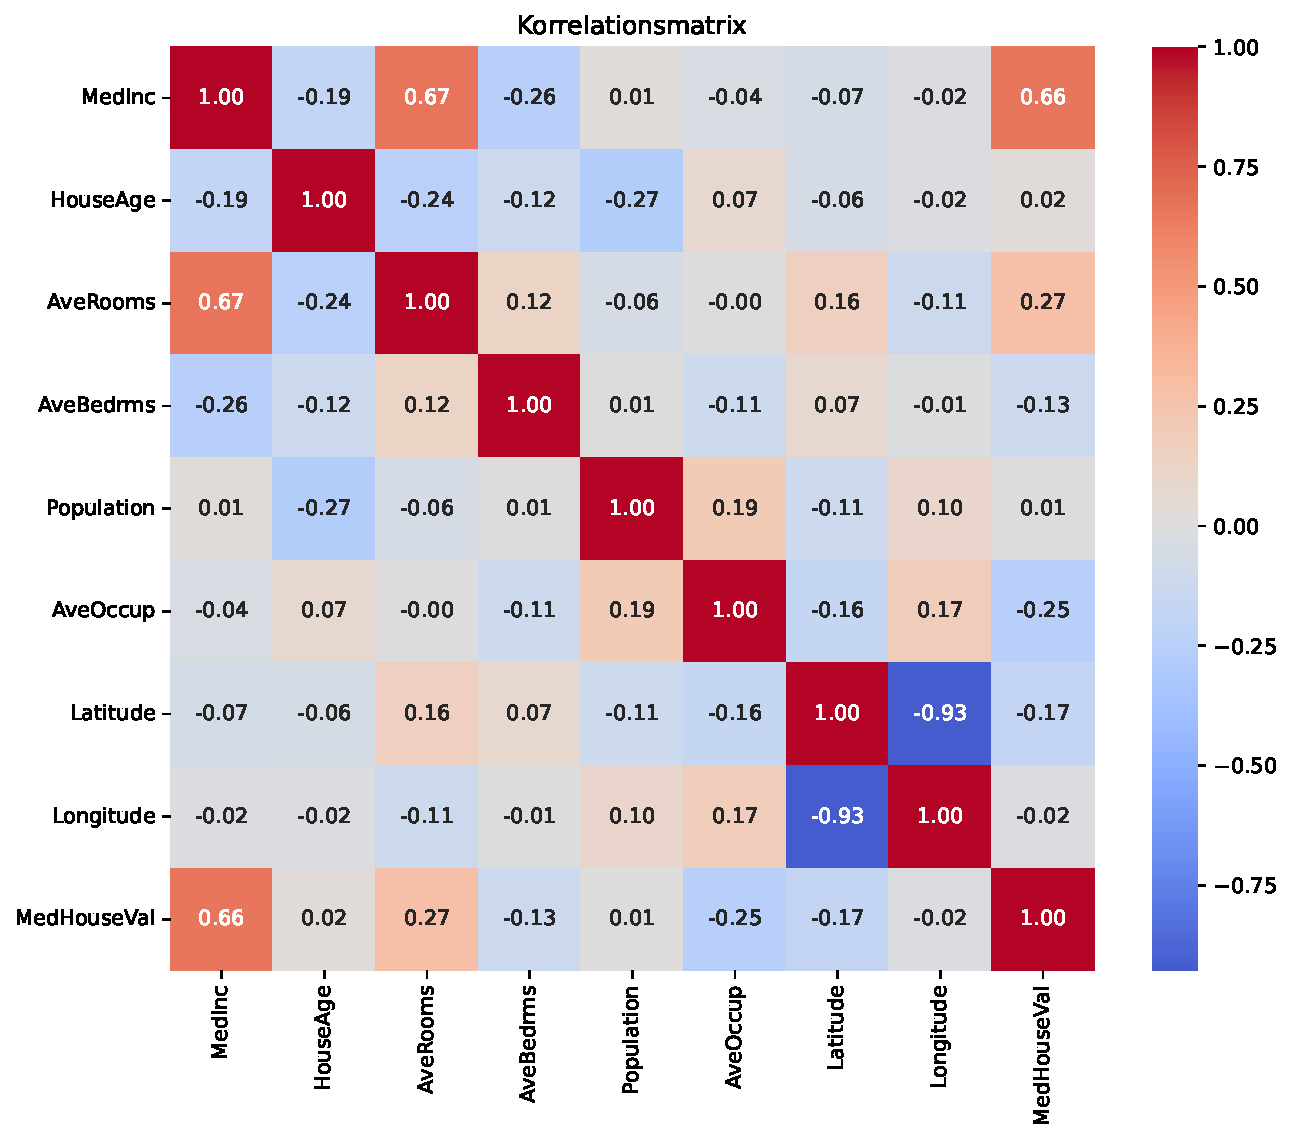
\includegraphics[width=0.95\columnwidth]{figures/eda_correlation_heatmap.pdf}
    \caption{Korrelationsmatrix der bereinigten Features. \texttt{MedInc} zeigt die st\"arkste Korrelation zur Zielvariablen \texttt{MedHouseVal}.}
    \label{fig:heatmap}
\end{figure}

\subsection{Baseline: Lineare Regression}

Als Referenzmodell dient eine lineare Regression auf allen 8~Features. Die Ergebnisse (\tabref{tab:results}) zeigen systematische Residuenmuster (\figref{fig:baseline}), die auf nichtlineare Zusammenh\"ange hindeuten, welche die lineare Regression nicht erfassen kann.

\begin{figure}[htbp]
    \centering
    %
\includegraphics[width=0.95\columnwidth]{figures/baseline_pred_vs_actual.pdf}
    \caption{Predicted vs.\ Actual f\"ur die lineare Regression. Die Streuung um die Diagonale und systematische Abweichungen bei hohen Preisen zeigen die Grenzen des linearen Modells.}
    \label{fig:baseline}
\end{figure}

\subsection{Neuronales Netz mit TensorFlow/Keras}

F\"ur das neuronale Netz habe ich systematisch verschiedene Architekturen getestet:

\begin{enumerate}
    \item \textbf{Modell~1:} [32] -- minimales Netz als Ausgangspunkt
    \item \textbf{Modell~2:} [64, 32, 16] -- tiefere Architektur
    \item \textbf{Modell~3:} [128, 64, 32] -- breiteres Netz
    \item \textbf{Modell~4:} Vergleich verschiedener Aktivierungsfunktionen (ReLU, ELU, tanh, sigmoid)
    \item \textbf{Modell~5:} [128, 64, 32, 16] + Dropout -- Regularisierung gegen Overfitting
\end{enumerate}

Alle Modelle wurden mit dem Adam-Optimizer (Lernrate 0{,}001) trainiert. Die Eingabedaten wurden standardskaliert, da neuronale Netze skalierte Features f\"ur effizientes Training ben\"otigen. \figref{fig:learning} zeigt die Lernkurven ausgew\"ahlter Modelle.

\begin{figure}[htbp]
    \centering
    %
\includegraphics[width=0.95\columnwidth]{figures/nn_learning_curves.pdf}
    \caption{Lernkurven (Loss und MAE) f\"ur verschiedene NN-Architekturen. Das Modell mit Dropout zeigt die stabilste Generalisierung.}
    \label{fig:learning}
\end{figure}

%----------------------------------------------------------

\section{Ergebnisse}

\tabref{tab:results} fasst die zentralen Ergebnisse zusammen. Das beste neuronale Netz (Modell~5: [128, 64, 32, 16] + Dropout) erreicht einen $R^2$-Wert von \textbf{0{,}78} auf dem Testset -- eine Verbesserung um 15~Prozentpunkte gegen\"uber der linearen Regression.

\begin{table}[htbp]
    \caption{Vergleich der Modellperformance auf dem Testset}
    \label{tab:results}
    \begin{tabular}{lccc}
        \toprule
        \textbf{Modell} & \textbf{$R^2$ Test} & \textbf{MAE} & \textbf{RMSE} \\
        \midrule
        Lineare Regression & 0{,}633 & 0{,}434 & 0{,}578 \\
        NN [32] & 0{,}712 & 0{,}362 & 0{,}512 \\
        NN [64, 32, 16] & 0{,}748 & 0{,}331 & 0{,}479 \\
        NN [128, 64, 32] & 0{,}726 & 0{,}345 & 0{,}499 \\
        \textbf{NN + Dropout} & \textbf{0{,}780} & \textbf{0{,}307} & \textbf{0{,}448} \\
        \bottomrule
    \end{tabular}
    \tabletext{MAE und RMSE in Einheiten von \$100.000. Das NN mit Dropout zeigt die beste Generalisierung.}
\end{table}

\figref{fig:comparison} visualisiert den direkten Vergleich: Das neuronale Netz zeigt eine engere Streuung um die Diagonale, insbesondere im mittleren Preissegment.

\begin{figure}[htbp]
    \centering
    %
\includegraphics[width=0.95\columnwidth]{figures/nn_vs_linear_regression.pdf}
    \caption{Kernvergleich: Lineare Regression (links) vs.\ bestes NN (rechts). Das NN approximiert die Diagonale deutlich besser.}
    \label{fig:comparison}
\end{figure}

\textbf{Zentrale Erkenntnisse:}
\begin{itemize}
    \item Das NN erfasst nichtlineare Interaktionen zwischen Features (z.\,B.\ Einkommen $\times$ Lage), die der linearen Regression verborgen bleiben.
    \item Ohne Regularisierung (Modell~3) tritt Overfitting auf: $R^2_{\text{Train}} = 0{,}88$ vs.\ $R^2_{\text{Test}} = 0{,}73$.
    \item Dropout (20\,\% in den ersten Schichten) reduziert die Generalisierungsl\"ucke effektiv.
    \item ReLU-Aktivierung liefert konsistent die besten Ergebnisse.
\end{itemize}

%----------------------------------------------------------

\section{Schwierigkeiten und Grenzen}

\subsection{Technische Herausforderungen}

\textbf{Python-Versionskonflikt:} TensorFlow~$\geq$~2.17 unterst\"utzt Python~3.14 nicht. L\"osung: Wechsel auf Python~3.13. F\"ur Teammitglieder mit Intel-Mac (TensorFlow-Inkompatibilit\"at ab 2.17) wurde Python~3.11 mit TensorFlow~2.16 als Alternative dokumentiert.

\textbf{Git-Workflow:} Mehrere Teammitglieder hatten Schwierigkeiten mit Git-Befehlen. Ich habe individuellen Support via Screensharing geleistet und \texttt{nbstripout} auf allen Systemen eingerichtet.

\subsection{Methodische Grenzen}

\begin{itemize}
    \item \textbf{Interpretierbarkeit:} Das NN ist eine Black Box -- f\"ur regulierte Dom\"anen (Kreditvergabe, Medizin) bleibt lineare Regression oft bevorzugt.
    \item \textbf{Hyperparameter-Tuning:} Architektur, Lernrate, Dropout-Rate, Epochenzahl -- der Suchraum ist gro{\ss}. Ein systematisches Grid-/Random-Search wurde noch nicht durchgef\"uhrt.
    \item \textbf{Rechenzeit:} Training auf CPU dauert ca.\ 1--2~Minuten pro Modell (300~Epochen). GPU-Beschleunigung w\"are f\"ur umfangreicheres Tuning sinnvoll.
\end{itemize}

%----------------------------------------------------------

\section{Zwischenstand und Ausblick}

Nach ca.\ 61~Stunden Arbeitszeit habe ich folgende Meilensteine erreicht:

\begin{enumerate}
    \item Vollst\"andige Projektinfrastruktur (Repository, Utils-Modul, 8~Notebooks)
    \item Explorative Datenanalyse und Baseline-Modell
    \item Systematischer Vergleich von 5~NN-Architekturen
    \item Git-Support f\"ur das gesamte Team
\end{enumerate}

\textbf{Offene n\"achste Schritte:}
\begin{itemize}
    \item Early Stopping zur automatischen Epochenwahl
    \item Learning-Rate-Scheduling f\"ur feineres Tuning
    \item Vergleich mit Ensemble-Methoden (Random Forest, Gradient Boosting) aus den Notebooks anderer Teammitglieder
    \item Feature-Engineering (Polynomiale Features, Interaktionsterme)
\end{itemize}

\textbf{Fazit:} Das neuronale Netz \"ubertrifft die lineare Regression deutlich und demonstriert die F\"ahigkeit, nichtlineare Muster im California-Housing-Datensatz zu lernen. Die Regularisierung durch Dropout ist essenziell f\"ur eine gute Generalisierung. Der erreichte $R^2$-Wert von 0{,}78 stellt einen soliden Zwischenstand dar, der durch weiteres Hyperparameter-Tuning noch verbessert werden k\"onnte.

%----------------------------------------------------------
\end{comment}
\printbibliography

%----------------------------------------------------------
\newpage
\section*{Einschätzung der Gruppenmitglieder}

\subsection{Name: Florian Adamczyk}
\paragraph{Stärken des Gruppenmitglieds}
    
\paragraph{Schwächen des Gruppenmitglieds}

\subsection{Name: Felix Hollfoth}
\paragraph{Stärken des Gruppenmitglieds}
\paragraph{Schwächen des Gruppenmitglieds}

\subsection{Name: Kolja Scriba}
\paragraph{Stärken des Gruppenmitglieds}
\paragraph{Schwächen des Gruppenmitglieds}

\subsection{Name: Björn Becker}
\paragraph{Stärken des Gruppenmitglieds}
\paragraph{Schwächen des Gruppenmitglieds}


\newpage 
%\includepdf[pages=-, link=true, linkname=logbuch]{Ergebnisse.pdf}
Platzhalter
\newpage
\section{Zusammenfassung der Gruppentreffen}
\newpage 
%\section*{Anhang: Logbuch}
% Der Parameter 'link=true' generiert automatisch Sprungmarken für jede Seite!
% 'linkname=logbuch' gibt diesen Seiten den Basisnamen "logbuch"
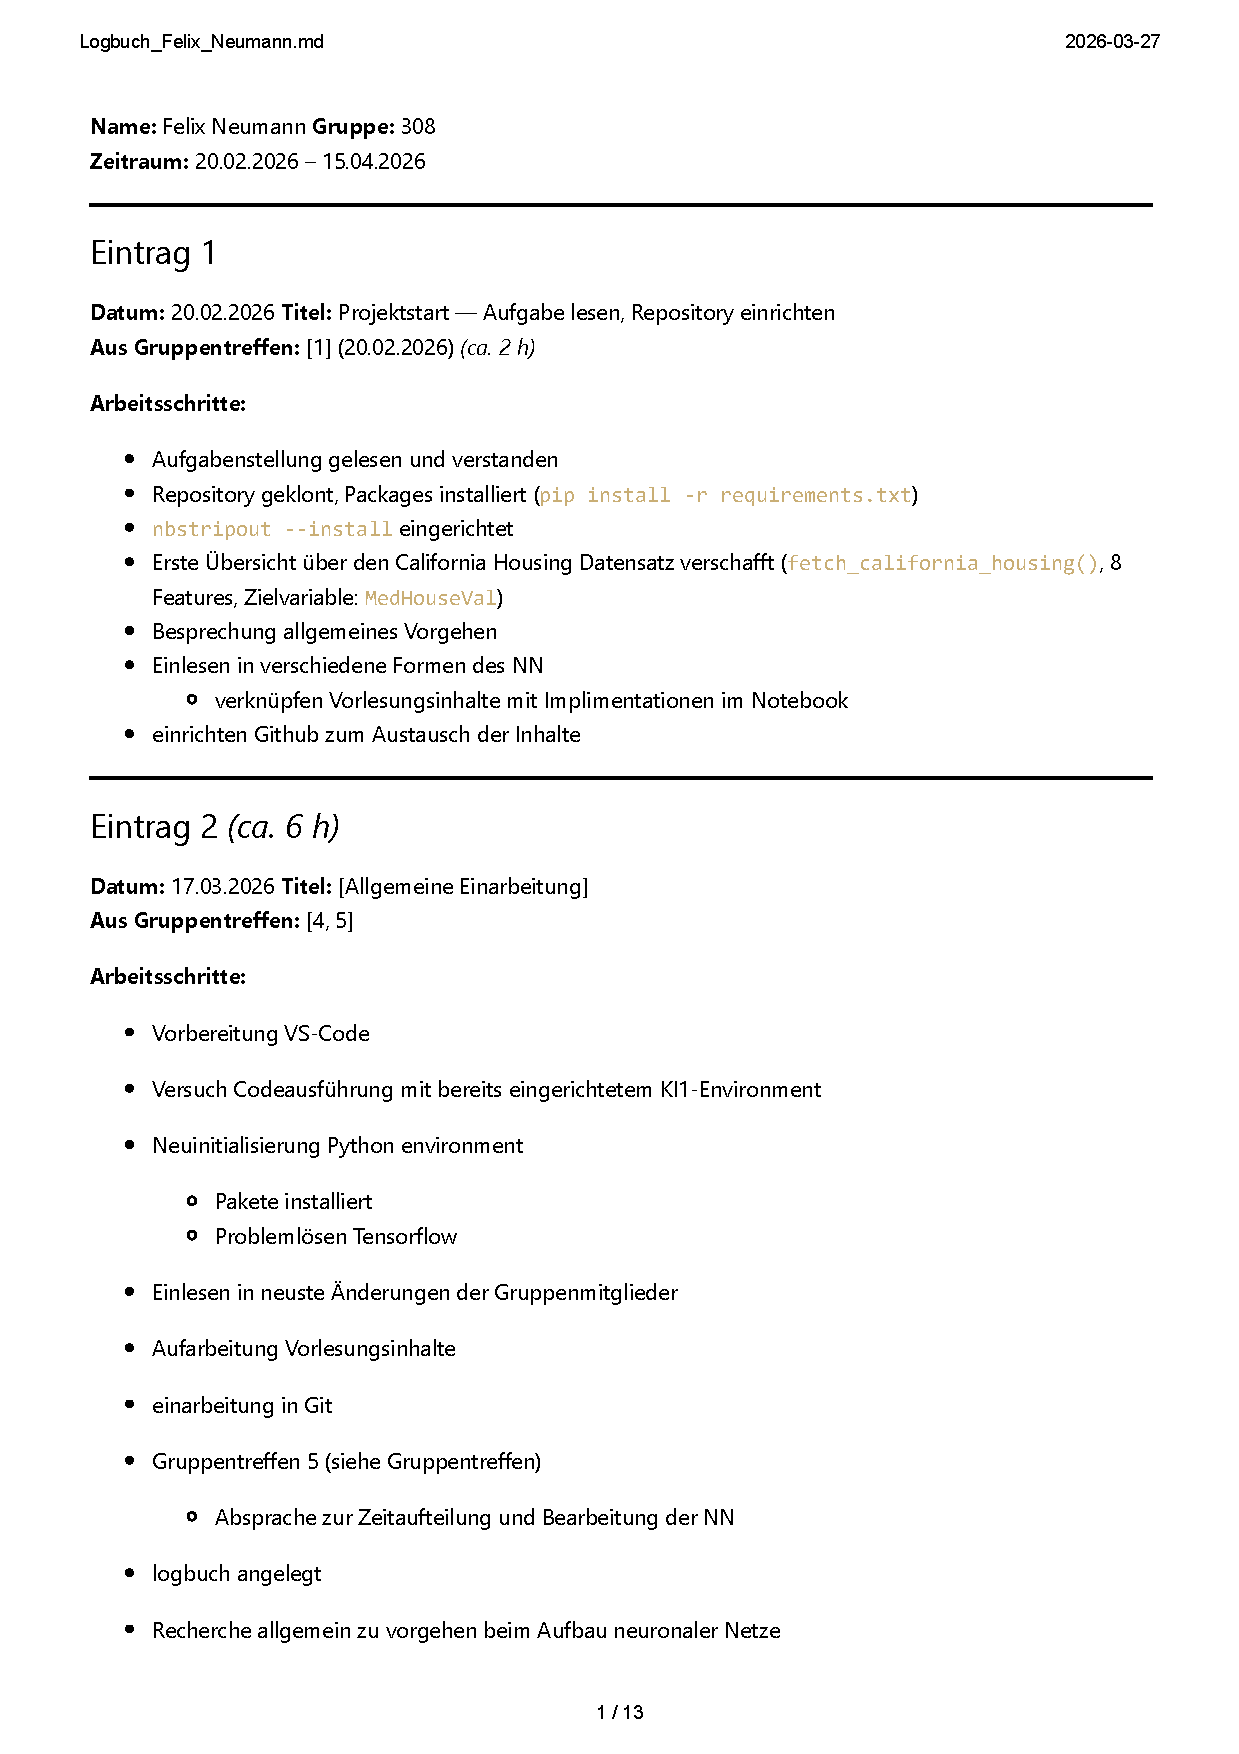
\includepdf[pages=-, link=true, linkname=logbuch]{Logbuch_Felix_Neumann.pdf}
%refernzieren auf Logbuch, siehe Anleitung
\end{document}
